%This file used to contain the geothermal chapter, now contains thermal/mechanical section of the conversion chapter
\section{Thermal Energy}
Thermal energy, or heat, can originate from many different sources including combustion of a fuel, radioactive decay, or absorption of light from the sun. Heat can be used directly to warm a building, but it is also a critical step in most traditional methods of generating electrical power. 
%\chapter{Geothermal Energy}
%\label{ch:geothermal}

\subsection{Enthalpy}
Enthalpy describes the energy of a system available to be converted to work. It is related to the temperature of the geothermal resource, but also dependent on the pressure and volume. Temperature is usually the primary metric of a resource, but even a high temperature source is useless without sufficient volume flow. Quantitatively enthalpy is expressed as 
\begin{equation}
H = U + pV
\end{equation}
where $U$ is the internal energy, which is function of temperature, $p$ is the pressure of the system, and $V$ is the volume. Generally it is more convenient to use the change in enthalpy rather than absolute values. After any a system undergoes some thermodynamic process the system will always have some remaining internal energy, pressure, and volume. Therefore a change in enthalpy better describes the energy extracted from (or absorbed by) the system.


\subsection{Geothermal Cycles}
%%Describe each of the following but focus on cycles for low enthalpy sources
Geothermal systems can be classified as high-, medium-, or low-enthalpy\footnote{While the technical definitions differ, the terms enthalpy, heat, and temperature are often used interchangeably when qualitatively describing geothermal sources.}. Although there is no formal delineation, high-enthalpy sources generally have temperatures greater than about $150$ \textcelsius{} ($302$ \textdegree{}F) and low-enthalpy sources have temperatures lower than $100$ \textcelsius{} ($212$ \textdegree{}F) \cite{Norden2011}. Depending on the amount of extractable energy of the resource, different geothermal processes or cycles should be used.

\subsubsection{Dry Steam}
This high-enthalpy processes extracts hot steam from the earth. The steam is sent directly through a turbine then condensed into liquid water and injected back underground. 

\subsubsection{Flash Steam} 
In the flash steam process high pressure hot is water extracted then allowed to boil becoming steam and low pressure hot water. The steam is sent through a turbine then condensed, recombined with water, and injected back underground.

\subsubsection{Binary Cycle} 
As the name implies, binary cycles involve two loops: a heat source loop and working fluid loop. Heat is collected in the heat source loop and transferred to the working loop through a heat exchanger. The working fluid then undergoes the vaporization process to spin a turbine or other type of expander. The expander is connected to a generator which converts the rotational mechanical energy into electrical energy. After some of the heat is converted, the working fluid passes through a condenser where it is cooled further. Sometimes the cooling process involves drawing in air at ambient temperature, but it can also involve a third loop. The fluids within each of the cycles each must be moved along using pumps. The pumps themselves need to be powered and act as a parasitic load to the system.

\begin{figure}[h]
	\centering

	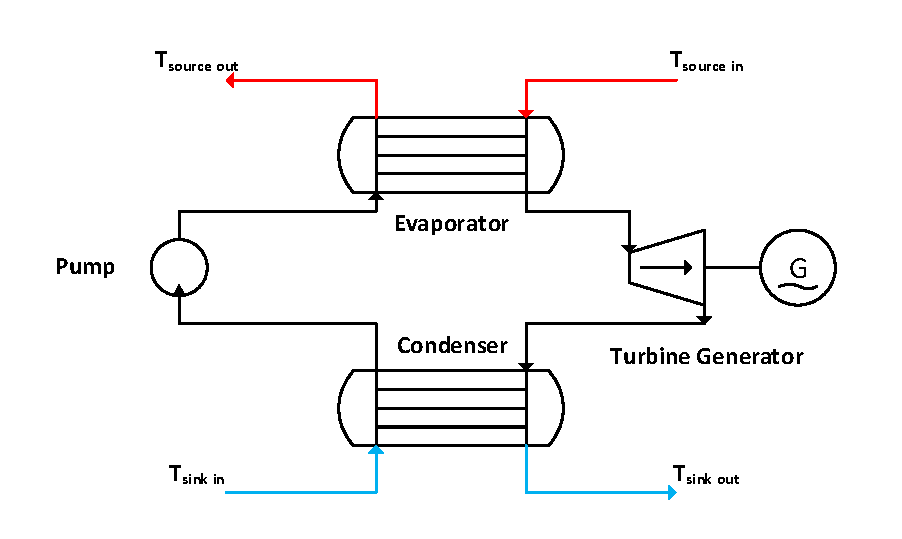
\includegraphics[width=\textwidth]{figures/RankineCycleDiagram.pdf}

	\caption{Diagram of a Rankine cycle system.}
	\label{fig:rankine_cycle_diagram}
	
\end{figure}

Binary cycles are not limited to low or medium enthalpy heat sources. The most common binary cycle is the Rankine Cycle. A diagram of the process can be seen in \autoref{fig:rankine_cycle_diagram}. In an ideal Rankine Cycle heat is added to the working fluid under high pressure to change its phase from liquid to gas. The fluid expands isentropically\footnote{In thermodynamics, isentropic processes do not have an net change in entropy} which rotates the generator shaft, causing the fluid's temperature and pressure drop. Additional heat is then expelled from the fluid as it condenses at a constant low pressure. Finally the fluid is isentropically pumped back to the high pressure and the process begins again.

For geothermal sources, generally high enthalpy systems can be implemented directly with a single loop using the flash or dry steam processes. However, for lower enthalpy systems, water cannot be used as a working fluid because the temperatures are not hot enough to vaporize it. In these cases an Organic Rankine Cycle can be used instead, which uses an organic working fluid such as refrigerants instead of water. Working fluids are typically selected for relatively low vaporization temperatures, but the thermodynamic states of the heat source also affect the choice. The selection of the type of expander and pumps are discussed in Kreider. \cite{Kreider} Generally larger diameter expanders operate at lower speeds.


%\subsubsection{(Organic) Rankine Cycle}
%\subsubsection{Kalina Cycle}




%\subsection{Pilgrim Hot Springs}
%Do this in 1st chapter not conv/geotherm chapter
%More thourough description of the resource and potential development plans.

\begin{comment}
\subsection{ORC Manufacturers and Developers}
A partial list of ORC system manufacturers and developers can be seen in \autoref{tab:orc_manufacturers}
\begin{table}
\centering
\caption{Manufacturers and developers of ORCs under development with less than ten documented installed systems. Also listed are the working fluids, mechanical drives, approximate rated operating speed, generator type, and rated output.}
\label{tab:orc_manufacturers_dev}
\rowcolors{1}{white}{gray!25}

\begin{tabular}[c]{p{2.7cm}p{2.8cm}p{2.0cm}p{1.5cm}p{1.6cm}p{2.0cm}}%{lllrlr}%
	\toprule
	%\multicolumn{6}{c}{ \multirow{2}{*}{\textbf{Under Development} (fewer than 10 documented installed systems)}}	\\ \midrule
	%\multicolumn{6}{c}{ \textbf{Under Development} (fewer than 10 documented installed systems)}	\\ \midrule
	%\multicolumn{6}{c}{}	\\ \hline
	%\rowcolor[gray]{5}
	\textbf{Company}		& \textbf{Working Fluid}		& \textbf{Mech. Drive} 		& \textbf{Rated RPM}	& \textbf{Gen. Type}	& \textbf{Size (kW)}  \\
	\midrule
	Air Squared				& 									& Scroll					& 2600 			& 						& 12 \\ 
	Termo2Power				& R245-fa							& Rotary Lobe				& 				& 						& \numrange{10}{300} \\ 
	Climeon					& 									& Turbine					& 				& 						& 150 \\ 
	Calnetix/ Access Energy	& R245-fa							& Turbine					& 30000			& PMSG					& 120 \\ 
	Verdicorp				&									& Turbine					& 45000			& PMSG 					& \numrange{65}{380} \\ 
	Inifinity Turbine		& R245-fa, supercrit. \ch{CO2}		& Radial Outflow Turbine	& 3600			& Induction \& DC 		& \numlist{10;50} \\ 
	Ener-G-Rotors			& 									& Trochoidal Gear Engine using ge-rotor &	&  						& \numlist{40;60} \\ 
	Phoenix					& R245-fa, Novec-649, Cyclohexane	& 							& 				& 						& \numlist{25;50;100;250} \\ \bottomrule
\end{tabular}
\end{table}
	
\begin{table}
\centering
\caption{Manufacturers and developers of commercial ORCs with more than ten documented installed systems. Also listed are the working fluids, mechanical drives, approximate rated operating speed, generator type, and rated output.}
\label{tab:orc_manufacturers_com}
\rowcolors{1}{white}{gray!25}	
\begin{tabular}[c]{p{3.0cm}p{2.5cm}p{2.0cm}p{1.5cm}p{1.6cm}p{2.0cm}}%{lllrlr}%
	\toprule
	\textbf{Company}          & \textbf{Working Fluid}		& \textbf{Mech. Drive}			& \textbf{Rated RPM}	& \textbf{Gen. Type}	& \textbf{Size (kW)}  \\
	\midrule
	Electratherm              & R245-fa 					& Twin Screw 					& 5000				& Induction  			& \numlist{35;65;110} \\ 
	E-Rationale               & R245-fa, SES36 				& Single Screw Radial Inflow	& 3600				& Induction				& \numlist{55;75;110;132} \\ 
	Exergy                    &								& Radial Outflow Turbine		&            		& 						& 125 and up \\ 
	Zuccato                   & Hydrofluoro-carbon mixture	& Radial Inflow Turbine			& 18000				& PMSG 					& \numlist{30;40;50} \\ 
	Enogia                    & R245-fa						& Turbine 						& 					& 						& \numlist{10;20;40;100}\\ 
	Clean Energy Technologies & R245-fa						& Turbine 						& 27500				& 						& 125 \\ 
	Tri-O-Gen                 & 							& Turbine 						& 					& 						& 165 \\ \bottomrule

\end{tabular}
\end{table}

\begin{comment}
%\subsection{ORC Manufacturers and Developers}
%\subsubsection{Under Development}
\begin{description}
	\item[Air Squared] Expander: Scroll expander based on automotive scroll compressor.
	\item[Termo2Power] Working fluid: R245fa. Expander: Rotary Lobe expander
	\item[Climeon] Expander: turbine expander.
	\item[Calnetix/Access Energy] Working fluid: R245fa. Expander: turbine expander
	\item[Verdicorp] has a range of variable speed expanders. The expander connects to the rotor of a permanent magnet synchronous generator. An IGBT variable frequency drive converts and synchronizes the power with a local grid. Expander: Turbine expander based on Dunfoss Turbocor compressor
	\item[Inifinity Turbine] 50kW Working fluid: R245fa -- 10kW Working fluid: supercritical $CO_2$. Expander: Radial Outflow Turbine
	\item[Ener-G-Rotors] Expander: Trochoidal Gear Engine using ge-rotor
	\item[Phoenix] Working fluid: R245fa
\end{description}
%\subsubsection{Commercial Products}
\begin{description}
	\item[Electratherm] makes use of a twin screw expander to spin an induction generator.  Working fluid: R245fa. Expander: Twin screw expander
	\item[E-Rationale] uses a single screw expander to rotate an induction generator. Working fluid: R245fa or SES36. Expander: Single screw expander
	\item[Exergy] Expander: Radial outflow turbine
	\item[Zuccato] uses a radial inflow turbine directly connected to synchronous permanent magnet generator. Electric power is converted and synchronized to local power grid with IGBT switching. Expander: Radial inflow turbine
	\item[Enogia] uses a turboexpander. Electric power is rectified then tied into the grid with a grid feed inverter. Working fluid: R245fa. Expander: Turbine expander
	\item[Clean Energy Technologies] %uses high speed turbine. Working fluid: R245fa. Expander: Turbine expander
	\item[Tri-O-Gen] %uses high speed turbine 
\end{description}
\end{comment} 


%\subsubsection{Under Development}
\begin{description}
\item[Air Squared] Expander: Scroll expander based on automotive scroll compressor.
\item[Termo2Power] Working fluid: R245fa. Expander: Rotary Lobe expander
\item[Climeon] Expander: turbine expander.
\item[Calnetix/Access Energy] Working fluid: R245fa. Expander: turbine expander
\item[Verdicorp] has a range of variable speed expanders. The expander connects to the rotor of a permanent magnet synchronous generator. An IGBT variable frequency drive converts and synchronizes the power with a local grid. Expander: Turbine expander based on Dunfoss Turbocor compressor
\item[Inifinity Turbine] 50kW Working fluid: R245fa -- 10kW Working fluid: supercritical $CO_2$. Expander: Radial Outflow Turbine
\item[Ener-G-Rotors] Expander: Trochoidal Gear Engine using ge-rotor
\item[Phoenix] Working fluid: R245fa
\end{description}
%\subsubsection{Commercial Products}
\begin{description}
\item[Electratherm] makes use of a twin screw expander to spin an induction generator.  Working fluid: R245fa. Expander: Twin screw expander
\item[E-Rationale] uses a single screw expander to rotate an induction generator. Working fluid: R245fa or SES36. Expander: Single screw expander
\item[Exergy] Expander: Radial outflow turbine
\item[Zuccato] uses a radial inflow turbine directly connected to synchronous permanent magnet generator. Electric power is converted and synchronized to local power grid with IGBT switching. Expander: Radial inflow turbine
\item[Enogia] uses a turboexpander. Electric power is rectified then tied into the grid with a grid feed inverter. Working fluid: R245fa. Expander: Turbine expander
\item[Clean Energy Technologies] %uses high speed turbine. Working fluid: R245fa. Expander: Turbine expander
\item[Tri-O-Gen] %uses high speed turbine 
\end{description}
\end{comment}

